%*******10********20********30********40********50********60********70********80

% For all chapters, use the newdefined chap{} instead of chapter{}
% This will make the text at the top-left of the page be the same as the chapter

\chap{Methodology}

\section{Overview}
To attain objective 1, our methodological approach consists in performing descriptive analysis of the network data of each co-authorship network, following the methodology used by Newman et al. \cite{newman_structure_2001} and Ghafouri et al. \cite{ghafouri_social_2014}. For objective 2, we use clustering methods, and shortest path algorithms as explained by Newman \cite{newman_scientific_2001,newman_scientific_2001-1}. Next, we apply mathematical modeling to attain objective 3. Regarding objective 4, we apply advanced statistical modeling including dynamic or longitudinal network analysis methods as recommended by Mali et al. \cite{mali_dynamic_2012}. We use a number of visualization methods to display the results. Finally, we develop a prototype of co-authorship tool to predict future research collaboration ties using the best performing statistical models. \\
The methodology workflow is presented in figure \ref{method_overview}.%we use link prediction as a topology inference method to predict future research collaboration ties.

%\begin{figure}[!ht]
\begin{sidewaysfigure}
\centering
%\begin{sidewaysfigure}
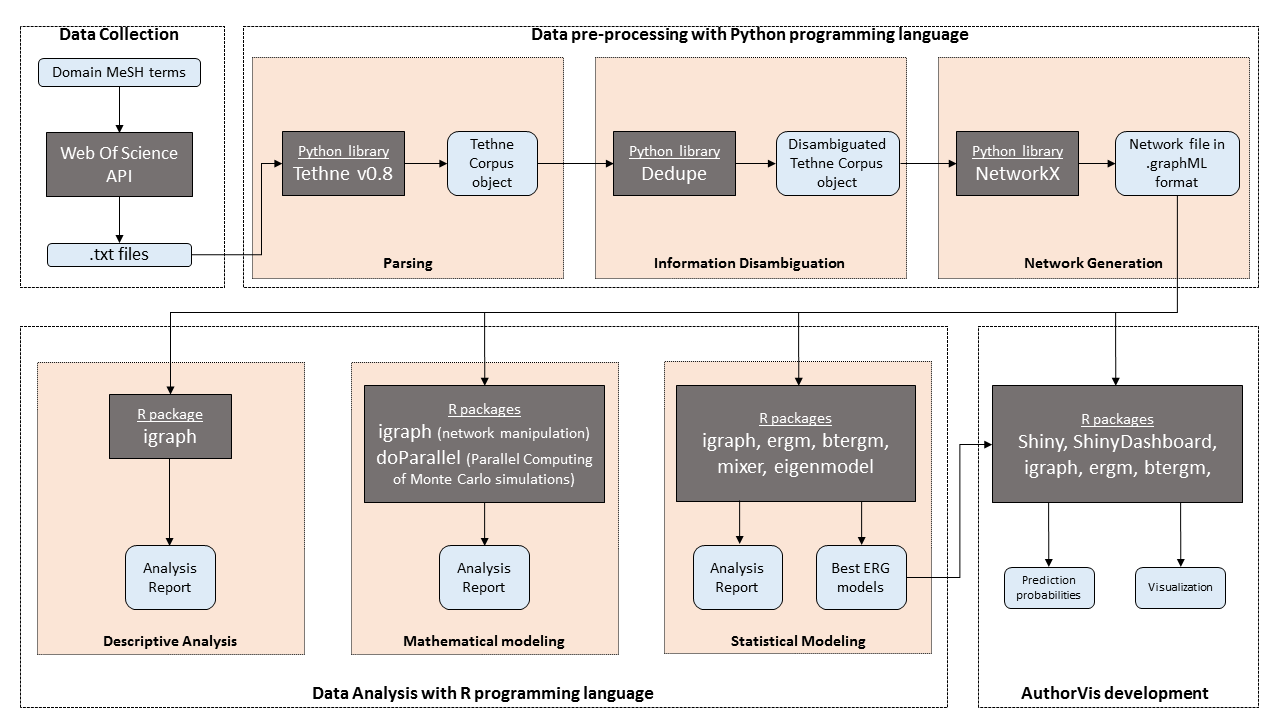
\includegraphics[scale=0.68]{Chapters/method_diagram}
%\end{sidewaysfigure}
\caption{Methodology Workflow}
\label{method_overview}
%\end{figure}
\end{sidewaysfigure}

\section{Data Collection}
\label{sec:data_collection}
Our research utilized secondary data collection techniques using the systematic literature search. We collected publication records indexed in the Thompson's Institute for Scientific Information Web Of Science (formerly known as the Web of Knowledge). %The search was conducted on papers published by Beninese authors, or papers published about Malaria, TB and HIV/AIDS involving authors affiliated to Beninese research institutions. Peer-reviewed articles were selected from systematic bibliographic search on papers indexed in Thompson's Institute for Scientific Information Web of Science (WOS) (formerly known as the Web of Knowledge). 
For each disease domain, we searched the WOS databases using combinations of disease related MeSH terms. For the malaria research domain, we combined the following MeSH terms: "Malaria", "Anopheles", "Plasmodium" and "vector". The HIV/AIDS  related MeSH terms are "HIV", "AIDS", "VIH", and "HIV infections". The TB related MeSH terms include "Tuberculosis", "Mycobacterium", and "Infection". We restricted the search to the period from 1996 to 2016 and to "Benin" for country. We manually screened the records in order to only select those published by Beninese authors, or papers published on each disease domain involving at least one author affiliated to a Beninese research institution. No restriction was placed upon the document types. For each disease domain, we first queried the WOS with each MeSH term independently, then combined the other terms so the query return the maximum number of results. The Full citations information containing the authors' names, their institutional affiliations, the year of publication, as well as the number of times the document was cited were recorded as bibliographic text files. After a second manual screening, only records that met the above listed inclusion criteria were finally selected. The selected records were saved in bibliographic text files and input to parser and functions for disambiguating the names of authors and other entities such as cities or research facilities.

\subsection{Parsing and Information Disambiguation}
\label{sec:meth_and}
%From each search domain, the bibliographic text files were parsed using Tethne v0.8 \cite{peirson_tethne_2016}, a python library for parsing bibliographic data. Tethne generated a bibliographic corpus object which is processed for information disambiguation.\\
%One common challenge in processing bibliometric data is the matching problem. Multiple names can refer to the same author. A well-known approach to solving this issue is termed as Author Name Disambiguation (AND). While many AND methods have been reported in the literature \cite{ferreira_brief_2012,giles_name_2005}, we chose to apply a fuzzy matching machine learning technique of AND. 
We used Dedupe, a python library (obtained from \url{https://github.com/datamade/dedupe}) to disambiguate authors' names and assign a unique identification number to each author. We manually annotated 10\% of the names and then trained the algorithm to automatically disambiguate the remaining of the entries. Dedupe is interactive and adjusts further annotations as the disambiguation process evolves. 
%Dedupe is based on the work of Bilenko \cite{bilenko_learnable_2006} and has been developed by Gregg Forest and Derek Eder. For more information on Dedupe, we refer the reader to the authors' Github repository available at \url{https://github.com/datamade/dedupe}.
We evaluated our AND fuzzy matching machine learning method by computing Precision and recall metrics. Dedupe was also used to normalize and disambiguate other information such as research center affiliations, city, and country. At the end of the Information Disambiguation process, a disambiguated Tethne corpus object was generated and used as input to the co-authorship network generation processing.
%The concept of AND has been extended to also disambiguate institution affiliation names and journal names. 


\subsection{Network Generation}
Using NetworkX \cite{schult_exploring_2008}, another python library, we wrote a script taking the disambiguated Tethne corpus object as input to generate undirected multigraph co-authorship networks containing parallel edges. Each author or researcher from the disambiguated Tethne corpus represented a vertex. An edge was created between two authors (vertices) when they author a document together. Multiple parallel edges were created between two authors when they coauthor multiple papers together. Our script output NetworkX graph objects where vertices were defined by several attributes including name, affiliation, city, country, number of publication and total number of times cited. Edges had attributes associated with them such as a unique identifier, the number of times a pair of authors was cited and the number of publications of a pair of authors. The undirected multigraph networkX objects were finally exported as .graphML files and used as input for data analyses.

%\section{Data Analysis}
\section{Descriptive Data Analysis}
For each co-authorship network, the numbers of authors, edges, and publications are plotted against the co-authorship years span. Using \textbf{igraph}, a network analysis package developed in R, each of the graphML files is converted into an igraph network object. For the descriptive analysis, we use the \textbf{igraph} package to compute the vertex degree and examined the degree distribution using both the natural frequency and the log scale degree distribution to characterize the type of distribution. We also computed vertex closeness, betweenness, eigenvector centrality measures and edge betweenness centrality measures to respectively identify the top 10 most connected authors, the top 10 broker authors, the top 10 network hubs, and the top 10 most important edges for information flow.  % and dyadic centrality measures:

%\begin{itemize}
%\item Degree of the vertices in the network defined as the number of ties to a given author. After converting the multigraph network in a weighted graph where weights are the number of authorship between two authors, the strength of the vertices was also computed.
%\item Betweenness: it is the number of shortest paths between alters that go through a particular author. It relates to the perspective that importance relates to where a vertex is located with respect to the paths in the network graph. According to Freeman \cite{freeman_set_1977}, it is defined as:
%\begin{equation} 
%c_{B}(v)=\frac{\sigma (s,t|v)}{\sum_{s \neq t \neq v \in V}\sigma (s,t)} 
%\end{equation} where $\sigma(s,t|v)$ is the total number of shortest paths between vertices $s$ and $t$ that pass through vertex $v$, and $\sigma (s,t)$ is the total number of shortest paths between $s$ and $t$ regardless of whether or not they pass through $v$.
%\item Closeness: the number of steps required for a particular author to access every other authors in the network. It captures the notion that a vertex is central if it is close to many other vertices. Considering a network $G=(V,E)$ where $V$ is the set of vertices and $E$, the set of edges, the closeness centrality $c_{Cl}(v)$ of a vertex $v$ is defined as:
%\begin{equation} c_{Cl}(v)=\frac{1}{\sum_{u\in V}dist(v,u)} \end{equation} where $dist(v,u)$ is defined as the geodesic distance between the vertices $u,v \in V$.
%\item Eigenvectors: degree to which an author is connected to other well connected authors in the network. It seeks to capture the idea that the more central the neighbors of a vertex are, the more central that vertex itself is. According to Bonacich \cite{bonacich_factoring_1972} and Katz \cite{katz_new_1953}, the Eigenvector centrality measure is defined as:
%\begin{equation} c_{E_i}(v)=\alpha \sum_{\{u,v\}\in E}c_{E_i}(u) \end{equation} Where the vector $\mathbf{c}_{E_i}=(c_{E_i}(1),\dots ,c_{E_i}(N_v))^T$ is the solution to the eigenvalue problem $\mathbf{Ac}_{E_i}=\alpha^{-1}\mathbf{c}_{E_i}$, where $\mathbf{A}$ is the adjacency matrix for the network $G$. According to Bonacich \cite{bonacich_factoring_1972}, an optimal choice of $\alpha^{-1}$ is the largest eigenvalue of $\mathbf{A}$
%\item Brokerage: degree to which an actor occupies a brokerage position across all pairs of alters.
%\item Edge betweenness centrality extends from the notion of vertex centrality. It reflects the number of shortest paths traversing that edge. This centrality measure was computed to assess which co-authorship collaboration ties are important for the flow of information.
%\end{itemize}

\subsection{Characterizing Network cohesion}
The extent to which subsets of authors are cohesive with respect to their relation in the co-authorship network was assessed through network cohesion. Specifically, we determined if collaborators (co-authors) of a given author tend to collaborate as well, and what subset of collaborating authors tend to be more productive in the network. 
%While there are many techniques to determine network cohesion \citep{kolaczyk_statistical_2014}, 
Using the \textbf{igraph} package, we conducted clique detection by computing the maximal cliques and their sizes, the density, and the transitivity. We also conducted a census of the connected components in each network, identify the giant component and characterize its size. Cut vertices were also computed to list the weak articulation points of each network. \\
The agglomerative hierarchical clustering method was used to identify clusters (or research communities) in the network. 
%In addition, we conducted cliques detection and clustering or communities detection on each network. 
Finally, we generated a visualization of each co-authorship network weighting the vertex size by their betweenness values and assigning colors based on their cluster membership determined by the hierarchical clustering method.
%\begin{itemize}
%\item Cliques: According to Kolaczyk and Cs\'ardi \cite{kolaczyk_statistical_2014}, cliques are defined as complete subgraphs such that all vertices within the subset are connected by edges. We computed the number of maximal cliques and assessed their size.
%\item Density: Defined as the frequency of realized edges relative to potential edges, the density of a subgraph $H$ in $G$ provides a measure of how close $H$ is to be a clique in $G$. Density values vary between 0 and 1:
%\begin{equation} 
%den(H)=\frac{|E_H|}{|V_H|(V_H-1)/2} 
%\end{equation}
%
%\item Relative frequency: we assess the relative frequency of $G$ by computing its transitivity defined as: 
%\begin{equation} 
%cl_T = \frac{3\tau_\Delta (G)}{\tau_3 (G)} 
%\end{equation}
%where $\tau_\Delta (G)$ is the number of triangles in $G$, and $\tau_3 (G)$ is the number of connected triples (sometimes referred to as 2-star). This measure is also referred to as the fraction of transitive triples. It represents a measure of global clustering of $G$ summarizing the relative frequency with which connected triples close to form triangles \cite{kolaczyk_statistical_2014}.
%\item Connectivity, Cuts, and Flows: We investigated the concepts of vertex and edge cuts derived from the concept of vertex (edge) connectivity. The vertex (edge) connectivity of a graph $G$ is the largest integer such that $G$ is k-vertex- (edge-) connected \cite{kolaczyk_statistical_2014}. These measures helped assess the most important authors for information flow and the long-term sustainability of each network. Since co-authorship networks are undirected graphs, the concept of weak and strong connectivity was irrelevant. A graph $G$ is said to be connected if every vertex in $G$ is reachable from every other vertex. Usually, one of the connected components can dominate the others, hence the concept of giant component.
%\item Graph Partitioning: Regularly framed as community detection problem, we applied graph partitioning to find subsets of vertices that demonstrate a 'cohesiveness' with respect to their underlying relational patterns. Cohesive subsets of vertices generally are well connected among themselves and are well separated from the other vertices in the graph. Two established methods of graph partitioning are Hierarchical clustering (agglomerative vs divisive) and Spectral clustering \cite{kolaczyk_statistical_2014}. In our research, we applied agglomerative Hierarchical Clustering to the co-authorship networks.
%\end{itemize}
\pagebreak
\section{Modeling of Network Data}
%The purposes of network graph modeling are to test significance of the characteristics of observed network graphs, and to study proposed mechanisms of real-world networks such as degree distributions and small-world effects \cite{kolaczyk_statistical_2014}. A model for a network graph is a collection of possible graphs $\mathscr{G}$ with a probability distribution $\mathbb{P}_\theta$ defined as:
%\begin{equation} 
%\{ \mathbb{P}_\theta\ (G), G \in \mathscr{G} : \theta \in \Theta \} 
%\end{equation}
%where $\theta$ is a vector of parameters ranging over values in $\Theta$.\\
%Given an observed co-authorship network graph $G^{obs}$ and some structural characteristics $\eta (\cdot)$, our goal is to assess if $\eta (G^{obs})$ is unusual. We then compare $\eta (G^{obs})$ to collection of values $\{\eta(G):G \in \mathscr{G}\}$. If $\eta (G^{obs})$ is too extreme with respect to this collection, then we have enough evidence to assert that $\eta (G^{obs})$ is not a uniform draw from $\mathscr{G}$.\\
%Given the computationally expensive calculations involved in modeling in general, and the expected large size of our network, we parallelized all processing.

\subsection{Mathematical Modeling}
%We used the characteristics of each observed network as input to the \textbf{igraph} package to simulate 1,000 networks from all four mathematical models for network graphs:
%\begin{itemize}
%\item Classical Random Graph Models: First established by Erd\H os and R\'enyi \cite{erdos_random_1959,erdos_evolution_1960,erdos_strength_1964}, it specifies a collection of graphs $\mathscr{G}$ with a uniform probability $\mathbb{P}(\cdot)$ over $\mathscr{G}$. A variant of this model called the Bernoulli Random Graph Model was also defined by Gilbert \cite{gilbert_random_1959}.
%\item Generalized Random Graph Models: These models emanated from the generalization of Erd\H os and R\'enyi's formulation, defining a collection of graphs $\mathscr{G}$ with prespecified degree sequence.
%\item Mechanistic Network Graph Models: These models mimic real-world phenomena and include Small-World Models commonly referred to as "six-degree separation". It was introduced by Watts and Strogatz \cite{watts_collective_1998} and have since received a lot of interests in the existing literature especially in Neuroscience. Small-world networks usually exhibit high levels of clustering and small distances between vertices. Classical models are not fit to better represent such behaviors since they usually display low levels of clustering and small distance between vertices. Examples of known small-world networks include the network of connected proteins  or the transcriptional networks of genes \cite{van_noort_yeast_2004}. A variant of Small-World models is the Preferential Attachment Models defined based on the popular principle of "the rich get richer". Preferential attachment models gained fascination after the work of Barab\'asi and Albert who studied the growth of the World Wide Web \cite{barabasi_emergence_1999}. Examples of Preferential Attachment networks include that of the World Wide Web and the scientific citation network \cite{albert_internet:_1999,jeong_measuring_2003}. An important characteristic of these models is that as time tend to infinity, there degree distribution tends to follow a power law.
%\end{itemize}
We input the observed characteristics of each co-authorship network to an \textbf{igraph} function to perform $1,000$ Monte-Carlo based simulations of the four different mathematical models for network graphs (Classical Random Graph, Generalized Random Graph, Watts-Strogatz Small-World, and the Barab\'asi-Albert Preferential Attachment) presented in section \ref{sec:back_mathModel}. We assessed the significance of the observed characteristics by comparing them to those of the $1,000$ simulated networks using a one sample Student’s t-test. Characteristics we assessed significance for are the average shortest paths, the clustering coefficient and the number of communities detected by the hierarchical clustering methods.

\subsection{Statistical Modeling}
%Although mathematical models tend to be simpler than statistical models, the latter allow model fitting and assessment. 
To model the complexity of the structure of each co-authorship network, we fit the SBM, the ERGM, the TERGM, and the LNM (presented in section \ref{sec:back_statModel}) to each co-authorship network data. 
For each model, we computed and included in the model an important social network principle referred to as homophily which is defined in our network as the tendency of similar authors to collaborate. Another very important social network principle we also computed and included in the model, is the one of structural equivalence which is the similarity of network positions on the formation of collaboration ties in a given network. 
%We hypothesized that tie formation in each co-authorship network (i) is dependent on certain authors' characteristics,  (ii) is dependent on the concept of distance in latent space, and (iii) collaboration type and/or membership to a certain research community or class determines collaboration tie formation. 
We used the results from the static and temporal statistical network models listed above to verify the hypotheses in section \ref{hypotheses}. The purpose of this approach to network modeling is to unveil structural patterns driving collaboration tie formation in each co-authorship network.

\subsubsection{Stochastic Block Model}
\label{sec:methods_sbm}
%Blockmodeling is a statistical method to identify, in a given network, clusters or classes of authors that share structural characteristics \cite{lorrain_structural_1971,doreian_generalized_2004}. Each such cluster forms a position. The units within a cluster have the same or similar connection patterns. Given a graph $G=(V,E)$ and its adjacency matrix $\mathbf{Y}$, for two distinct nodes $i,j \in V$, the block model defined by Kolaczyk and Cs\'ardi \cite{kolaczyk_statistical_2014}, specifies that each element $Y_{ij}$ of $\mathbf{Y}$ is conditional on the class label $q$ and $r$ of the vertices $i$ and $j$. The model has the form:
%\begin{equation}Pr(\mathbf{Y}=\mathbf{y})=\left( \frac{1}{\kappa} \right) exp \set*{ \sum_{q,r} \theta_{qr} L_{qr}(\mathbf{y}) }\end{equation}
%where $L_{qr}$ is the number of edges in the observed graph $\mathbf{y}$ connecting vertices of classes $q$ and $r$, $\theta_{qr}$ is the parameter estimates, and $\kappa$ is a normalization constant defined as:
%\begin{equation}
%\kappa = \sum_{\mathbf{y}}exp \set*{ \sum_{q,r} \theta_{qr} L_{qr}(\mathbf{y}) }
%\end{equation}
%Stochastic block model (SBM) originated from the ideas that equivalent units can be grouped together. There are three definitions of equivalences which are structural, automorphic and regular \cite{mali_dynamic_2012}. In practice, the differences in types of equivalence tend to blur when stochastic block modeling is applied to real networks. 
We used SBM to both model each of the observed networks but also as a model based clustering technique. After fitting the SBM, we examined the posterior probability of class membership from the returned object. We then determined the class membership of each vertex class assignment based on the maximum a posteriori criterion. Class membership was added to the network as an additional nodal attribute. Subroutines of R package \textbf{mixer} \citep{Daudinmixturemodelrandom2008,ZanghiFastonlinegraph2008,ZanghiStrategiesonlineinference2010,LatoucheVariationalBayesianinference2012} was used to fit and evaluate the SBM. \textbf{Mixer} used the Integration Classification Likelihood (ICL) criterion to select the number of classes fit to the observed network. We finally examined the summary plot generated by the \textbf{Mixer} package which contains the ICL, the degree distribution, the reorganized adjacency matrix, and the inter/intra class probability plots. While the ICL plot displays the optimal number of classes, the degree distribution helps assess the goodness-of-fit of the SBM to the observed data. The reorganized adjacency matrix plot shows the interactions between the classes of the network and the inter/intra class probabilities plot highlights the inter and intra interactions between the detected classes.
%
%\subsubsection{Dynamic Stochastic Block Model}
%\label{sec:methods_dynsbm}
%The Dynamic Stochastic Block Model (dynSBM) emerged from the recent interests in statistical modeling of dynamic or temporal networks \cite{xu_dynamic_2014}. It is a recent model based clustering approach to dynamically evolving or longitudinal networks \cite{matias_statistical_2016,hutchison_dynamic_2013,xu_dynamic_2014}. We refer the reader to the work of Matias and Miele \cite{matias_statistical_2016} in their 2016 paper for a thorough model definition.\\ 
%The dynSBM method is a combination of Stochastic Block Model (SBM) \cite{kolaczyk_statistical_2009} described in section \ref{sec:methods_sbm} for the static aspect and independent Markov chains for the temporal evolution of the network. The main focus of this method is on nodes classification or the task of community detection. The dynSBM method allows the modeling of sequence of different snapshots of temporal or dynamic networks. In a different paper, the method was used to unveil the dynamic structure of different ecologic networks of colonies of ants or a community of Broadstone Stream \cite{miele_revealing_2017}. The model is suited for discrete time in dynamic networks. We used dynSBM to investigate research group switching across the investigation period, and map the dynamic of collaborative research among the identified research groups. We presented an alluvial plot representing a map of the co-authorship patterns, group switching within time. The R package \textbf{dynSBM} \cite{matias_statistical_2016} was used to fit the dynSBM. Matias and Miele \cite{matias_statistical_2016} assert that the number of groups can be selected statistically using the Integration Classification Likelihood (ICL) criterion or the "elbow" heuristic. The optimum number of groups therefore corresponds to the highest ICL. As per the "elbow" heuristic, the optimum number of groups corresponds to the point where the slope of the log-likelihood decreases significantly. In this thesis, we used both the ICL and the "elbow" heuristic to select the number of groups in the final dynSBM model. We defined the selected number of detected groups in the final model as the minimum of the number of detected groups determined by the ICL criterion and the "elbow" heuristic.

\subsubsection{Exponential Random Graph Model}
\label{sec:methods_ergm}
%Also referred to as p* models, Exponential Random Graph Models (ERGMs) are probability models for network designed in analogy to Generalized Linear Models (GLMs) \cite{kolaczyk_statistical_2014}. ERGMs have gain increasing interests especially in modeling social networks. Robins et al. \cite{robins_introduction_2007} provides a nice introduction to ERGM as well as a general framework for ERGM creation which we closely followed here. 
The R package \textbf{ergm} \cite{HandcockERGMFitsimulate2003,HunterergmPackageFit2008} was used to fit ERGM to the observed networks. We used ERGM to model the network ties, the dependent variable as a function of nodal and dyadic attributes (covariates) such as the number of times an author was cited, the number of publications, the number of collaborators, the collaboration type as well as its community membership as determined by the SBM. \\
%investigate how local processes affect collaboration tie formation between authors. We 
Given the high transitivity coefficient of this network, we also included transitivity as a network structural process. As recommended for ERGM model specification for undirected network, we investigated homophily which is the tendency of similar author to collaborate. We also included factor attribute effect in the model. \\
%Given a random graph $G=(V,E)$, for two distinct nodes $i,j \in V$, we define a random binary variable $Y_{ij}$ such that $Y_{ij}=1$ if there is an edge $e \in E$ between $i$ and $j$, and $Y_{ij}=0$ otherwise. Since co-authorship networks are by definition undirected networks, $Y_{ij}=Y_{ji}$ and the matrix $\mathbf{Y}=\left[Y_{ij}\right]$ represents the random adjacency matrix for $G$. The general formulation of ERGM is therefore:
%\begin{equation}
%Pr(\mathbf{Y}=\mathbf{y})=\left( \frac{1}{\kappa} \right) exp \set*{ \sum_{H} \theta_H g_H(\mathbf{y})}
%\end{equation}
%where each $H$ is a configuration, a set of possible edges among a subset of the vertices in $G$ and $g_H(\mathbf{y})=\prod_{y_{ij} \in H}y_{ij}$ is the network statistic corresponding to the configuration $H$; $g_H(\mathbf{y})=1$ if the configuration is observed in the network $\mathbf{y}$, and is $0$ otherwise. $\theta_H$ is the parameter corresponding to the configuration $H$ (and is non-zero only if all pairs of variables in $H$ are assumed to be conditionally dependent); $\kappa$ is a normalization constant defined as:
%\begin{equation}
%\kappa = \sum_{\mathbf{y}}exp \set*{ \sum_{H} \theta_H g_H(\mathbf{y})}
%\end{equation}.\\
Several models containing nodal, dyadic and structural terms were fit to the observed network data. The first model we fit is a naive model containing only the ERGM "edge" term. This model is nothing but the Bernoulli random graph model \cite{erdos_random_1959}. We then fit another model containing only nodal and/or dyadic terms. Third, we fit a structural model containing only high-order terms representing network statistics such as triangles, k-stars, geometrically weighted edge-wise shared partner distribution and many more \cite{kolaczyk_statistical_2014,robins_introduction_2007}. \\
%Ideally, we expect the best model to contain nodal and dyadic covariates as well as high order ERGM terms. 
Model log-likelihood, the Akaike's Information (AIC) and the Bayesian Information (BIC) criteria were used to select the best ERGM. The best model was selected based on the lowest AIC, or the lowest BIC, and the highest log-likelihood. Usually, AIC and BIC decrease or increase together. In case of conflicting trend in AIC and BIC values, the log-likelihood was used to select the best model. We checked for model diagnostics by computing and inspecting the Goodness-Of-Fit visualization for the best model using a subroutine of the \textbf{ergm} package. %generated whenever necessay, we finally evaluated the best model (lowest AIC or BIC and highest likelihood) by assessing its goodness-of-fit to the observed network. 
A maximum of 1,000 iterations and 1,000 simulations was set as parameters to the ERGMs.

\subsubsection{Temporal Exponential Random Graph Model}
\label{sec:methods_tergm}
All Temporal Exponential Random Graph Models (TERGMs) were fit using the Markov Chain Monte Carlo Maximum Likelihood Estimation (MCMC-MLE) implemented in the \textbf{btergm} R package \cite{leifeld_temporal_2015}. 
%The Temporal Exponential Random Graph Model (TERGM) is an extension of the ERGM described in section \ref{sec:methods_ergm} proposed by Hanneke, Fu, and Xing \cite{hanneke_discrete_2010} from the work of Robins and Pattison \cite{robins_random_2001}. The TERGM was designed with the idea of accounting for inter-temporal dependence in longitudinally collected network data. TERGM was applied to each co-authorship network following from the work of Leifeld, Cranmer, and Desmarais \cite{leifeld_temporal_2015}. For a full description of the TERGM, we refer the reader to Leifeld, Cranmer, and Desmarais \cite{leifeld_temporal_2015}. \\
%Each network is subset in different temporal snapshots. In general, when the temporal network is overly dense or sparse early on or in later time periods, the TERGM tends to fit different time spans differently \cite{leifeld_temporal_2015}. To avoid such an issue, the cumulative network was subset in a certain way that balanced the number of edges across the years. 
%This strategy improved the robustness and convergence of our models. %--->this goes to the discussion
We divided each network in different snapshots spanning different intervals of time using a manual process such that the temporal snapshots are not overly dense or sparse early on or in later time periods. We used \textbf{igraph} to visualize and manually verified that the temporal snapshots are balanced across the time periods. We then modeled the network ties, the dependent variable as a function of nodal and dyadic variables. Dyadic stability and delay reciprocity memory TERGM terms were also included in the model. To check whether there is a linear trend in collaboration tie formation, we also included a linear time covariate in the model. We accounted for network structural predictors and homophily on the type of collaboration.  Model log-likelihood, the Akaike's Information (AIC) and the Bayesian Information (BIC) criteria were used to select the best TERGM corresponding to the lowest AIC or BIC, and highest log-likelihood. AIC and BIC are estimates of a function of the posterior probability of a model being true. Under a Bayesian setup, a lower BIC or AIC means that a model is more likely to be the true model.  \\
To evaluate the extent to which the final model captures the endogenous properties and processes of the observed network, we assessed model diagnostics, by inspecting the within-sample and out-of-sample goodness-of-fit visualization computed from a subroutine of the \textbf{btergm} package. For the out-of-sample goodness-of-fit, we estimated the model on the first network snapshots leaving out the last network snapshot in the series. We simulated $1,000$ networks from the model and assessed how the simulated networks predicted the left out network. As described by Desmarais and Cranmer \cite{desmarais_micro-level_2012}, we also provided a micro-interpretation of the final TERGM.

\subsubsection{Latent Network Model}
\label{sec:methods_lnm}
%Designed in analogy to Mixed Models, Latent Network Models (LNM) allow the incorporation of latent or unobserved variables in network modeling. These models specifically account for structural equivalence, to model hidden factors or information not available in the network. Kolaczyk and Cs\'ardi \cite{kolaczyk_statistical_2014} provide a formulation of LNM. Given the adjacency matrix $\mathbf{Y}$ of a graph $G=(V,E)$, for each element $Y_{ij}$ of $\mathbf{Y}$, the latent variable model is of the form:
%\begin{equation}Y_{ij}=h(\theta,z_i,z_j,\epsilon_{ij})\end{equation} where $\theta$ is a constant, the $\epsilon_{ij}$ are independent and identically distributed pair-specific effects, and $h$ is a symmetric function. The model assumes that each vertex $i\in V$ has a latent variable $z_i$. Considering observed covariates $\mathbf{Z}$, the probability of forming an edge between two nodes $i$ and $j$ ($i,j \in V$) is independent of all other vertex pairs given values of latent variables, and is defined as:
%\begin{equation}
%Pr(\mathbf{Y}|\mathbf{Z},\theta)=\prod_{i\neq j}Pr\left(Y_{ij}|z_i,z_j,\theta \right)
%\end{equation}
Hoff \cite{hoff_modeling_2008} suggested an approach based upon the principles of eigen-analysis of specifying latent variables which we followed in this dissertation. The R package \textbf{eigenmodel} developed by Hoff \cite{hoff_eigenmodel:_2012} was used to fit the LNM to the observed networks. We fit LNM with both no pair-specific and pair-specific covariates such as the type of collaboration and community assignment from the SBM. The rationale of fitting the pair-specific models with those two variables is supported by our third hypothesis which states that collaboration ties in each co-authorship network are driven by homophily in terms of community membership and/or collaboration type. We also fit other pair-specific covariates model using nodal and dyadic covariates. We visualized and compared the co-authorship network using 3 dimensional layouts determined according to the inferred latent eigenvectors in each model. Finally, we used a 5-fold cross-validation method to assess the goodness-of-fit of each model which we compared using ROC curves via the R package \textbf{ROCR} \citep{SingROCRvisualizingclassifier2005}.\\
~\\
The creation of the co-authorship tool is presented in Chapter \ref{chap_authorvis}.


%\section{Research Collaboration Ties Prediction}
%Collaboration recommendation has already been identified as valuable for interdisciplinary research, encouraging joint research and cross-domain collaboration efforts \cite{tang_cross-domain_2012,trujillo_collaboration_2010}. Often, such collaborations are hard to researchers to establish. Link prediction effectively addresses the issue of link recommendation as one of the network topology inference questions. The link prediction question as formalized by Liben-Nowell and Kleinberg \cite{liben-nowell_link-prediction_2007} seeks to infer new future interactions among members of a social network given a snapshot of such network. After developing and proposing several approaches to the link prediction question, their first application was on large co-authorship networks. Unlike many other networks, co-authorship networks are dynamic in nature. New authors can make their apparition in the network while old authors may disappear. New authorship collaborations may be initiated while old ones may stop.\\
%The many approaches to the link prediction problem can be classified in three main techniques: (i) Node neighborhood, (ii) Path based technique, and (iii) Distance based technique \cite{sharma_link_2014}. Different predictors defined each of those link prediction techniques. For example, Jaccard-coefficient, Adamic-Adar and preferential attachment are node neighborhood predictors while examples of path based predictors are Katz, and rooted PageRank.\\ 
%We used Linkpred, an easy link prediction tool written in Python and available at \url{https://github.com/rafguns/linkpred}. Our choice of this tool is motivated by the fact it is based on machine learning and uses a wide range of global, local and distance based predictors.
%Our goal was to predict future co-authorship links in 5 and 2 years based on the observed collaboration over a 20 years of research collaboration. We therefore split each network data in a training set and a test set. Prediction models were trained on the training set and evaluated on the test set. In the 5-year link prediction question, we inferred new collaborations between authors in the next 5 years. Hence, our training set covered the first 15 years and the test set, the next 5 years. Similarly, for the 2-year link prediction question, we split the data in a training set covering the first 18 years and a test set of the next 2 years for evaluation purposes.\\
%The Receiver Operating Curve (ROC), the Area Under the Curve (AUC), precision, recall and F-measures were used as evaluation metrics.
